\documentclass[10pt,a4paper]{article}
\usepackage[margin=22mm]{geometry}
\usepackage[T1]{fontenc}
\usepackage{lmodern,amsmath,amssymb,booktabs,graphicx,tikz,hyperref,fvextra}
\usetikzlibrary{arrows.meta,positioning,calc,decorations.pathmorphing}
\definecolor{ink}{RGB}{20,53,78}
\hypersetup{colorlinks=true,urlcolor=ink,linkcolor=ink}
\setlength{\parindent}{0pt}
\setlength{\parskip}{5pt}
\emergencystretch=3em

\title{\color{ink}A precision platform under floor motion}
\author{}
\date{Original learning collection -- November 2026}
\begin{document}
\begin{center}{\LARGE\color{ink}A precision platform under floor motion}\\[5pt]{\small Original learning collection -- November 2026}\end{center}

\textbf{Evidence note.} Original teaching scenario. Numerical parameters are deliberately chosen for learning. All generated data and curves are synthetic; no physical measurement is asserted.
\section{Design brief}
An optical platform has mass $m=8\,\mathrm{kg}$ and spring stiffness $k=3200\,\mathrm{N/m}$. Compare damping ratios $\zeta=0.08$ and $0.40$. Derive transmissibility from floor coordinate $z$ to absolute platform coordinate $x$, find the isolation threshold and compare attenuation at $\omega=2\omega_n$. Also find the displacement produced by a static $1\,\mathrm{N}$ force.
\section{Physical system}
\begin{center}\resizebox{\ifdim\width>.98\linewidth.98\linewidth\else\width\fi}{!}{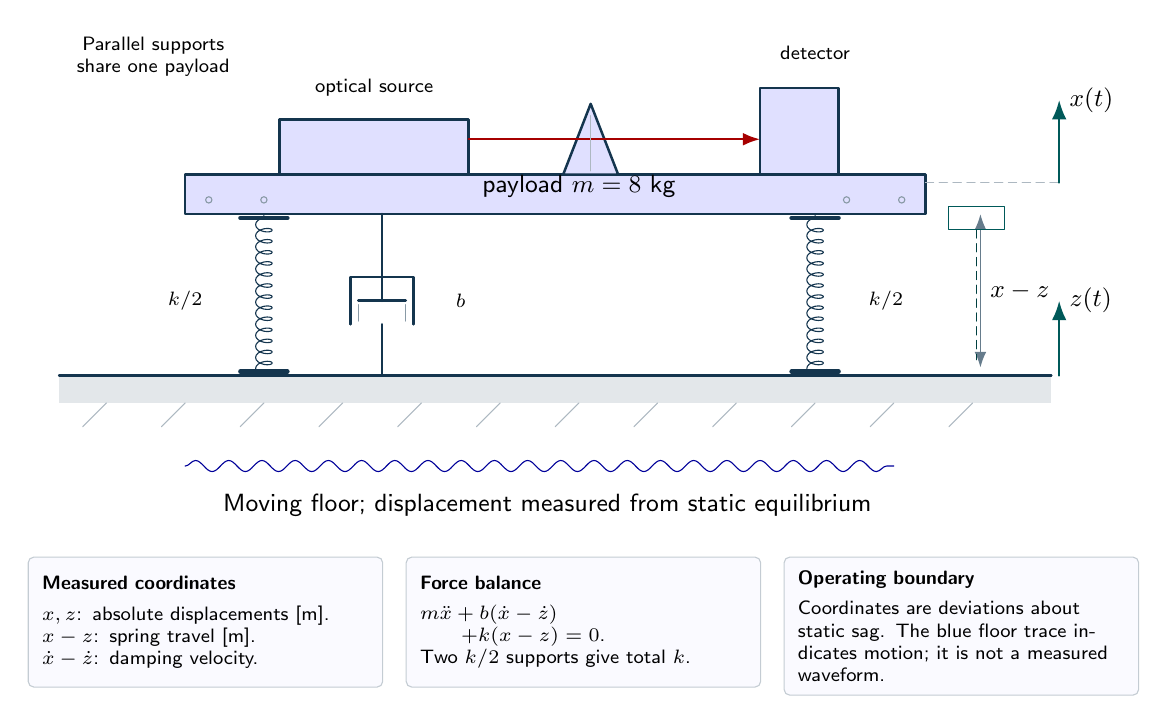
\begin{tikzpicture}[
font=\sffamily\small,>=Latex,line cap=round,line join=round,
wall/.style={draw=ink,line width=1.2pt,fill=blue!5},
water/.style={fill=cyan!25,draw=none},
metal/.style={draw=ink,fill=blue!12,line width=.9pt},
flow/.style={->,draw=blue!65!black,line width=1.2pt},
heat/.style={->,draw=orange!85!black,line width=1.1pt},
measure/.style={->,draw=teal!70!black,line width=.9pt},
dim/.style={<->,draw=ink!65,line width=.6pt},
spring/.style={draw=ink,decorate,decoration={coil,aspect=.5,segment length=4pt,amplitude=3pt}},
wire/.style={draw=ink,line width=1pt},
lab/.style={align=center,font=\sffamily\small},
smalllab/.style={align=center,font=\sffamily\scriptsize}]

\fill[ink!12](.4,.2)rectangle(13,.55);
\draw[ink,line width=1pt](.4,.55)--(13,.55);
\foreach \x in {1,2,...,12}{\draw[ink!35](\x,.2)--++(-.3,-.3);}
\draw[metal](2,2.6)rectangle(11.4,3.1);
\draw[spring](3,.55)--(3,2.6);
\draw[spring](10,.55)--(10,2.6);
\draw[wire](4.5,.55)--(4.5,1.2)(4.1,1.2)--(4.1,1.8)--(4.9,1.8)--(4.9,1.2);
\draw[wire](4.5,2.6)--(4.5,1.5)(4.2,1.5)--(4.8,1.5);
\draw[metal](3.2,3.1)rectangle(5.6,3.8);
\draw[metal](6.8,3.1)--(7.15,4)--(7.5,3.1)--cycle;
\draw[metal](9.3,3.1)rectangle(10.3,4.2);
\draw[red!65!black,->,line width=.7pt](5.6,3.55)--(9.3,3.55);
\node[smalllab]at(4.4,4.2){optical source};
\node[smalllab]at(10,4.65){detector};
\node[lab]at(7,2.95){payload $m=8$ kg};
\node[smalllab]at(2,1.5){$k/2$};\node[smalllab]at(10.9,1.5){$k/2$};
\node[smalllab]at(5.5,1.5){$b$};
\draw[dim](12.1,.65)--node[right]{$x-z$}(12.1,2.6);
\draw[ink!35,densely dashed](11.4,3)--(13.1,3);
\draw[measure](13.1,3)--(13.1,4.05)node[right]{$x(t)$};
\draw[measure](13.1,.55)--(13.1,1.5)node[right]{$z(t)$};
\draw[blue!60!black,decorate,decoration={snake,amplitude=2pt,segment length=12pt}](2,-.6)--(11,-.6);
\node[lab]at(6.6,-1.1){Moving floor; displacement measured from static equilibrium};
% REFINED EQUIPMENT DETAILS

% Fasteners, spring seats and a clearly resolved dashpot piston.
\foreach \x in {2.3,3,10.4,11.1}{\draw[ink!50](\x,2.78)circle(.04);}
\foreach \x in {3,10}{\draw[ink,line width=1.5pt](\x-.3,.6)--(\x+.3,.6)(\x-.3,2.55)--(\x+.3,2.55);}
\draw[ink!50](4.2,1.24)--(4.2,1.45)(4.8,1.24)--(4.8,1.45);
\draw[ink!35](7.15,3.15)--(7.15,3.85);
\draw[teal!70!black](11.7,2.4)rectangle(12.4,2.7);
\draw[teal!50!black,densely dashed](12.05,2.4)--(12.05,.75);
\node[smalllab,anchor=west]at(.5,4.6){Parallel supports\\share one payload};

\node[draw=ink!25,fill=blue!2,rounded corners=2pt,anchor=north west,text width=4.15cm,minimum height=1.65cm,inner sep=5pt,align=left,font=\sffamily\scriptsize]at(0.0,-1.75){\textbf{Measured coordinates}\\[3pt]$x,z$: absolute displacements [m].\\$x-z$: spring travel [m].\\$\dot x-\dot z$: damping velocity.};
\node[draw=ink!25,fill=blue!2,rounded corners=2pt,anchor=north west,text width=4.15cm,minimum height=1.65cm,inner sep=5pt,align=left,font=\sffamily\scriptsize]at(4.8,-1.75){\textbf{Force balance}\\[3pt]$m\ddot x+b(\dot x-\dot z)$\\$\qquad+k(x-z)=0$.\\Two $k/2$ supports give total $k$.};
\node[draw=ink!25,fill=blue!2,rounded corners=2pt,anchor=north west,text width=4.15cm,minimum height=1.65cm,inner sep=5pt,align=left,font=\sffamily\scriptsize]at(9.6,-1.75){\textbf{Operating boundary}\\[3pt]Coordinates are deviations about static sag. The blue floor trace indicates motion; it is not a measured waveform.};
\end{tikzpicture}
}\par{\small An optical payload rests on parallel spring and damping elements. The two springs each have stiffness $k/2$, giving total $k$. Both the floor and payload move; spring extension and damping velocity are relative quantities. Weight is balanced at the static equilibrium about which the model is written.}\end{center}
\section{Relative forces, absolute displacement}
Let $x$ be platform displacement and $z$ floor displacement. The spring and damper act on relative motion:
\[m\ddot x=-b(\dot x-\dot z)-k(x-z)+f.\]
Thus the floor and force inputs have different numerators:
\[\frac{X}{Z}=\frac{bs+k}{ms^2+bs+k},\qquad \frac{X}{F}=\frac1{ms^2+bs+k}.\]
With $m=8$ kg and $k=3200$ N/m, $\omega_n=20$ rad/s and $b=2\zeta\sqrt{mk}=320\zeta$ N s/m. The two damping values are 25.6 and 128 N s/m.
\section{Transmissibility and isolation}
For $r=\omega/\omega_n$, the squared displacement transmissibility is
\[|X/Z|^2=\frac{1+(2\zeta r)^2}{(1-r^2)^2+(2\zeta r)^2}.\]
It is below one precisely when $(1-r^2)^2>1$, or $r>\sqrt2$ for positive frequency. Damping does not move this crossing, but it changes resonance and high-frequency transmission.
\section{A design tradeoff}
At $r=2$, use $\sqrt{[1+16\zeta^2]/[9+16\zeta^2]}$. Greater damping lowers resonance but increases transmission in the isolation band. A static 1 N force produces $x=1/k=0.0003125$ m irrespective of damping.
\section{Limits}
The floor is an imposed displacement, not a second independent mass. Mount stiffness and damping are ideal constants; travel limits, friction, rotations and material nonlinearities are excluded.
\section{What to learn from the experiment}
Reducing a resonance peak and improving high-frequency isolation are different design objectives. The transfer function must reflect which physical input is applied.
\section{System sketch}
\begin{center}\resizebox{\ifdim\width>.98\linewidth.98\linewidth\else\width\fi}{!}{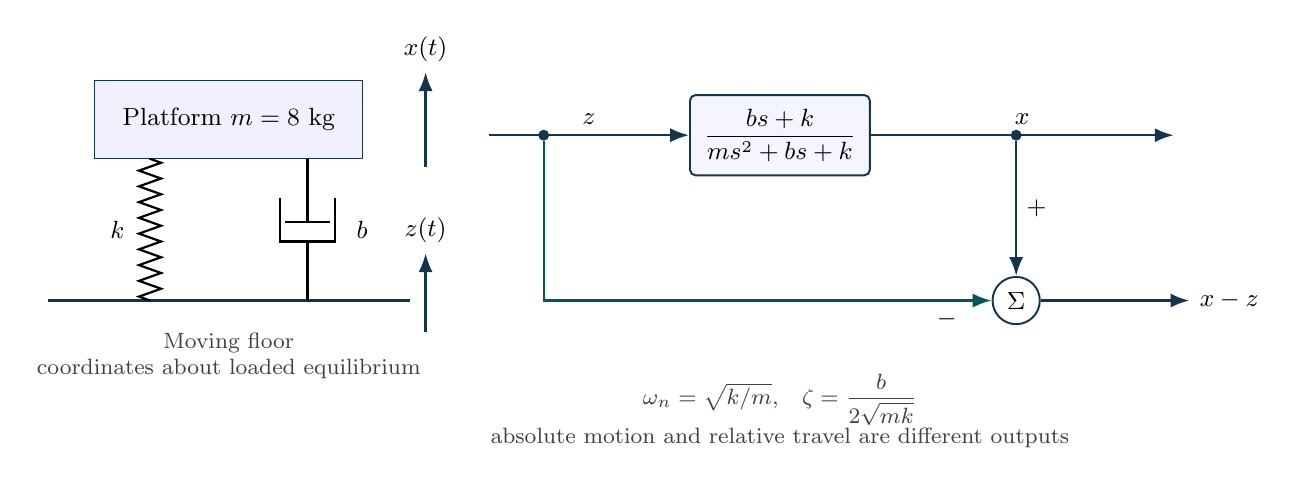
\begin{tikzpicture}[x=1cm,y=1cm,>=Latex,font=\small,
block/.style={draw=ink,fill=blue!4,rounded corners=2pt,minimum height=9mm,align=center,line width=.7pt,inner sep=5pt},
sum/.style={circle,draw=ink,fill=white,minimum size=6mm,inner sep=0pt,line width=.7pt},
sig/.style={->,draw=ink,line width=.85pt},
fb/.style={->,draw=teal!70!black,line width=.85pt},
dist/.style={->,draw=orange!75!black,line width=.85pt},
tap/.style={circle,fill=ink,inner sep=1.4pt},
note/.style={font=\footnotesize,align=center,text=black!75}]

\node[draw=ink,fill=blue!6,minimum width=34mm,minimum height=10mm](m)at(2,2.2){Platform $m=8$ kg};
\draw[line width=1.2pt,draw=ink](-.3,-.1)--(4.3,-.1);
\draw[decorate,decoration={zigzag,segment length=2mm,amplitude=1.4mm},line width=.8pt](1,-.1)--(1,1.7);
\node[left]at(.8,.8){$k$};
\draw[line width=.8pt](3,-.1)--(3,.65);
\draw[line width=.8pt](2.65,1.2)--(2.65,.65)--(3.35,.65)--(3.35,1.2);
\draw[line width=.8pt](2.72,.9)--(3.28,.9);
\draw[line width=.8pt](3,.9)--(3,1.7);
\node[right]at(3.5,.8){$b$};
\draw[sig](4.5,1.6)--(4.5,2.8)node[above]{$x(t)$};
\draw[sig](4.5,-.5)--(4.5,.5)node[above]{$z(t)$};
\node[note]at(2,-.8){Moving floor\\coordinates about loaded equilibrium};
\node[block](g)at(9,2){$\dfrac{bs+k}{ms^2+bs+k}$};
\node[tap](zt)at(6,2){};
\node[tap](xt)at(12,2){};
\draw[sig](5.3,2)--node[above]{$z$}(g);
\draw[sig](g)--node[above]{$x$}(14,2);
\node[sum](rel)at(12,-.1){$\Sigma$};
\draw[sig](xt)--node[right]{$+$}(rel);
\draw[fb](zt)--(6,-.1)--node[pos=.9,below]{$-$}(rel);
\draw[sig](rel)--(14.2,-.1)node[right]{$x-z$};
\node[note]at(9,-1.5){$\omega_n=\sqrt{k/m}$,\quad $\zeta=\dfrac{b}{2\sqrt{mk}}$\\absolute motion and relative travel are different outputs};

\end{tikzpicture}
}
\par\small\refstepcounter{figure}\label{fig:system}\textbf{Figure \thefigure.} Base excitation drives absolute motion; subtracting the floor coordinate gives relative travel. The spring and damper act in parallel.\end{center}
\section{Executed computational evidence}
\VerbatimInput[fontsize=\small,breaklines=true]{results.txt}
\begin{center}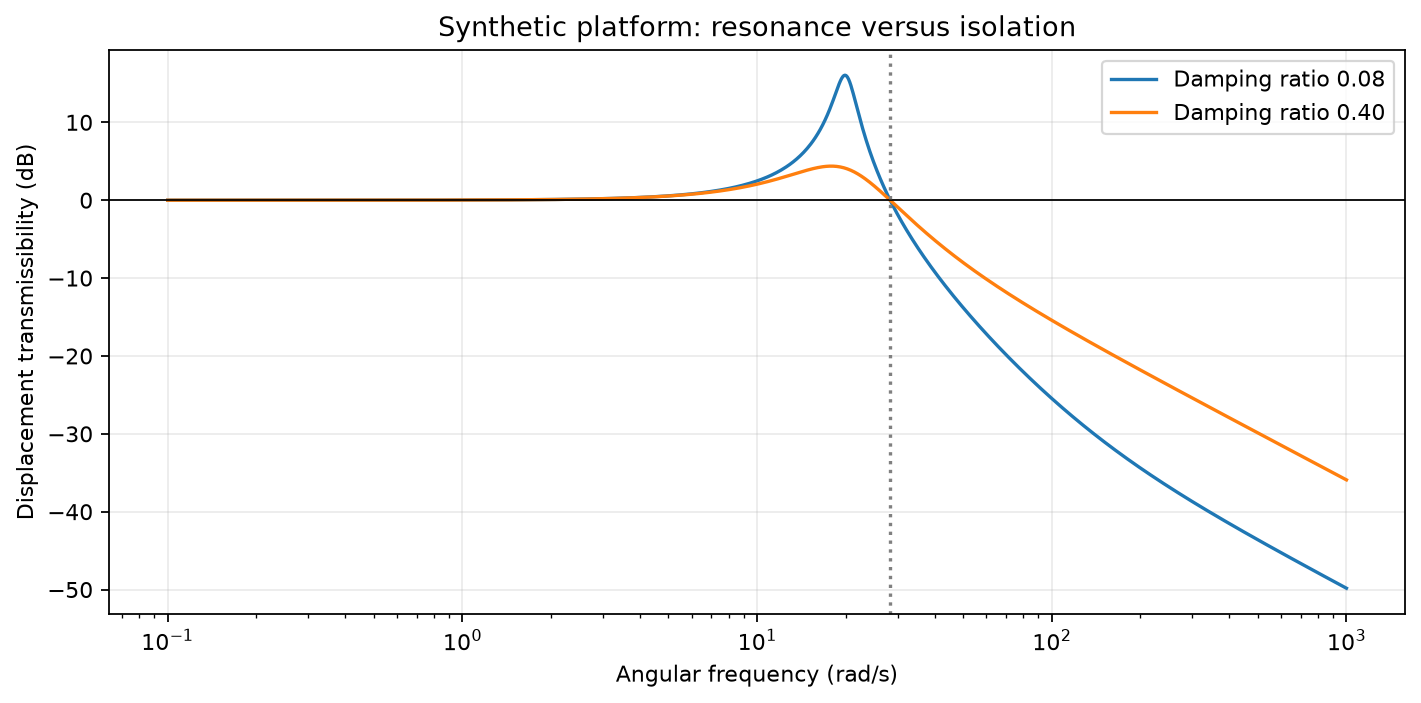
\includegraphics[width=\linewidth,height=.46\textheight,keepaspectratio]{response.png}\end{center}
\section{Method references}
The equations use standard balance laws and feedback-control methods. Further explanation: \url{https://apmonitor.com/pdc/} and \url{https://fbsbook.org/}. Implementation documentation: \url{https://python-control.readthedocs.io/en/0.10.2/}. See the repository reference catalog for individual topics and videos.
\end{document}
